\renewcommand{\thechapter}{\Roman{chapter}}
\chapter{Introduction}
\renewcommand{\thechapter}{\arabic{chapter}}
\label{ch:Introduction}
\thispagestyle{empty}

\section{Background of the Study}
\label{intro:sec:Background of the Study}

Agricultural raw materials, such as rice, wheat, and corn, which mostly include solid, liquid or powered, provide significant amounts of carbohydrates for use in industry and human nutrition . Certain grains require little processing and can be eaten right away after harvest, while others must be prepared through a number of primary and secondary milling steps. As farmers learned to produced more resulting of various agricultural innovation, this raw materials must preserve the quality for future consumption \citep{Bucklin2019175}.
It is expected an increase in raw materials annually does necessitate an efficient post-harvest processes such as raw product storing method incorporating modern technologies \citep{yegorova_2021}.

Various tools and methods have been developed to measure stored raw materials volume inside an industrial storage silos or bins, employing sensors like contact level indicators (e.g., tilt switches, pressure diaphragms, rotary paddles) and non-contact indicators (e.g., stereovision, radar, ultrasound, lasers). Contact sensors offer cost-effective, dust-resistant point measurements but lack surface detail. Non-contact sensors can map grain surfaces accurately but require permanent mounting, are relatively expensive, and are susceptible to dust interference. However, conventional volumetric measurement method using weighted fiberglass tape is still being used providing only a single data point which leads to inaccuracy and error-prone volume measurement \citep{turner2017}.

Point cloud data consists of a set of points representing an object in either a two or three-dimensional structure. This data typically comprises X, Y, and Z coordinates, but modern point clouds may also include additional information such as intensity, RGB values, and more \citep{wang2019306, stojanovic2023point}.

Light Detection and Ranging (LiDAR) is one of the many devices that can gather 3D points that often refer as point clouds. Unfortunately, commercial 3D LiDAR systems tend to be expensive in comparison to their 2D-based LiDAR. This cost disparity can lead to limitations in accessibility for certain applications or industries, hindering widespread adoption and innovation in fields where 3D spatial data is crucial. Low-cost two axes-based LiDAR can mimic the collection of 3D point cloud by adding an additional axes using tilting device \citep{clar2022}. However, it comes with a notable drawback: it lacks several capabilities present in high-end 3D LiDAR systems, including multi-echo functionality, long-range detection, high angular resolution, among others.

Recent innovations in various industries have made the production less manual but producing more by using automation and wireless technologies that helped to produce better and accurate measurement compared to traditional methods. These approaches include various sensing technologies, automated measurements, machine to machine (M2M) communications, and monitoring systems. The interconnected sensors and actuators allow to remotely collect data, store, and process the data to provide better insight in the industry and also for the economic growth, specify the characteristics of a paperless factory, it is a development of a smart factory in which all data that is turned into information is stored, transferred, and displayed entirely remotely and digitally. As the level of digitization of a smart factory, it is not a revolution but rather an evolution \citep{bulut2020}.

%Although laser  technology have been proved to be useful and excellent in various field compared to other technology with in terms of its capabilities, features, and accuracy, however, it produced undesirable or no data when the environment is exposed to dust or fog the blocks the visibility of the object interest \citep{yigit2015,turner2017,duysak2020}. With the given circumstances, todays commercial high-end LiDAR still gather relevant data to analyze using multi-echo functionality and some hardware improvement which, unfortunately, lacks on low-cost LiDAR.

\section{Statement of the Problem}
\label{intro:sec:Statement of the Problem}
%A variety of product that stored in a silo can be solid, powdered and liquid. When the product such as solid grains, corn are being stored, minimal dust cloud are generated during filling process. However, when powdered products such as cement or flour are being filled, a dense dust cloud are created. Ideally, when LiDAR is used for measuring the distance between the product and the door, it is installed at the top. Due to the fine-texture of solid materials such as flour product, a dispersed dust cloud may form during the pneumatic conveying process of loading flour into the bin \citep{williams2007}. Although LiDAR sensor have the ability to provide faster data collection and detailed spatial illustration compared to other sensing technologies, and the precision of distance measurement is undeniable, the wavelengths that LiDAR operates, typically, 700 to 900 nm can be problematic when deposit layers of dust formed caused by stored product as it may caused a problem when scanning the spatial structure of the product.

While some food manufacturing industries still rely on manual and labor-intensive storage measurement procedures, there is a growing need to adopt advanced technologies with remote capabilities. This shift aims to eliminate the need for frequent physical processes that may endanger employees. Silo storage systems are versatile, accommodating a wide range of products, including solids, powders, and liquids. One characteristic of product storages is that when they are filled with raw materials, except for liquids, they create a dust cloud in the empty space. Solid grains like corn typically produce minimal dust clouds during filling, whereas powdered substances like cement or flour often generate dense dust clouds.

When implementing LiDAR for storage volume measurement, the ideal placement is at the top of the silo. However, in the case of fine-textured solid materials such as flour, dispersed dust clouds may arise during the pneumatic conveying process of loading flour into the bin \citep{williams2007}. Although LiDAR sensors offer advantages such as rapid data collection and precise spatial representation compared to alternative sensing technologies, their operational wavelengths—usually between 700 to 900 nm—can pose challenges when scanning through layers of dust deposited by stored products. This challenge may potentially impact the accuracy of spatial structure scans.

This study presents the development of a 3D point cloud scanner system for volume measurement of flour storage. The system is designed to be controlled and scanned remotely, alleviating the manual process of volume measurement. Additionally, this study investigates the behavior of the system when dust clouds are present during filling.

%There are various advanced LiDAR technologies such as 3D LiDAR sensors that are available in the market, primarily used for robotics applications, that can address these problems without the need of additional hardware and software configuration. However such sensing devices are too expensive and sophisticated. The focus of this study is to utilized low-cost LiDAR technology to partially mimic the sophisticated functionality of the above mentioned technology.

\section{Objectives of the Study}
\label{intro:sec:Objectives of the Study}
The general objective of this study was to develop a system that can remotely measure the volume of the product inside of a flour storage bin using point cloud data and Web-based Application. The following specific goals were completed:

\begin{enumerate}
	\item Designed and developed a 3D point cloud scanner system (3D-PCSS);
	\item Developed a web-based application for remote access and visualization of the system;
	\item Tested and evaluated the performance of the system.
\end{enumerate}

\section{Originality of the Study}
\label{intro:sec:Originality of the Study}
The originality of this study lies in the development of a system capable of remotely estimating and monitoring the volume and capacity of storage materials. This study introduces two distinct components: the point cloud acquisition system and the web application system designed for remote monitoring purposes. Furthermore, the study explores the system's behavior in the presence of dust, providing insights for further enhancement and modification.

\section{Scope and Limitations}
\label{intro:sec:Scope and Limitations}
The scope of this study is to develop a volume estimation system through remote point cloud acquisition and a web application. It is important to note that the system testing was not conducted directly in a commercial manufacturing industry or an actual industrial storage bin. Instead, testing took place in an open area using a mock-up storage bin designed to replicate the size and shape of a typical industrial storage facility. Additionally, the study exclusively focuses on utilizing flour as the primary raw material for testing purposes.


\section{Significance of the Study}
\label{intro:sec:Significance of the Study}
Accurate and efficient post-harvest processes is vital in the food industry to ensure effective inventory management and maintain an adequate supply of materials. Automation with remote sensing devices are modern technologies that can be integrated to a variety of industry, eliminating labor-intensive that may exposed employees to a dangerous scenarios. The study was able to  However, when flour is involved, dust clouds can form inside the bin during scanning, potentially leading to inaccurate data from the 3D point cloud scanner. Such inaccuracies can impact subsequent processing of the point cloud data. Therefore, the findings of this study hold significance in several key areas:

\begin{description}
	\item[Industrial Automation:] This study utilizes remote sensing technology, specifically LiDAR, to automate the volume estimation process for flour bins. The developed method has the potential to reduce the need for manual measurements, enhancing both the accuracy and efficiency of volume measurements in industrial settings.

	\item[Point Cloud Processing:] The study focuses on the development of an automated volume measurement method for flour bins based on 3D point cloud data. A point cloud is a collection of data points in a 3D space, obtainable using various sensors like LiDAR. The study's central contribution lies in its processing of the point cloud, a critical step that involves manipulating, analyzing, and interpreting 3D point cloud data. The results of this study will enrich the field of knowledge related to point cloud processing techniques, benefiting industries beyond just flour bin volume estimation.
\end{description}

\section{Conceptual Framework}
\label{intro:sec:Conceptual Framework}

\begin{figure}[H]
	\centering
	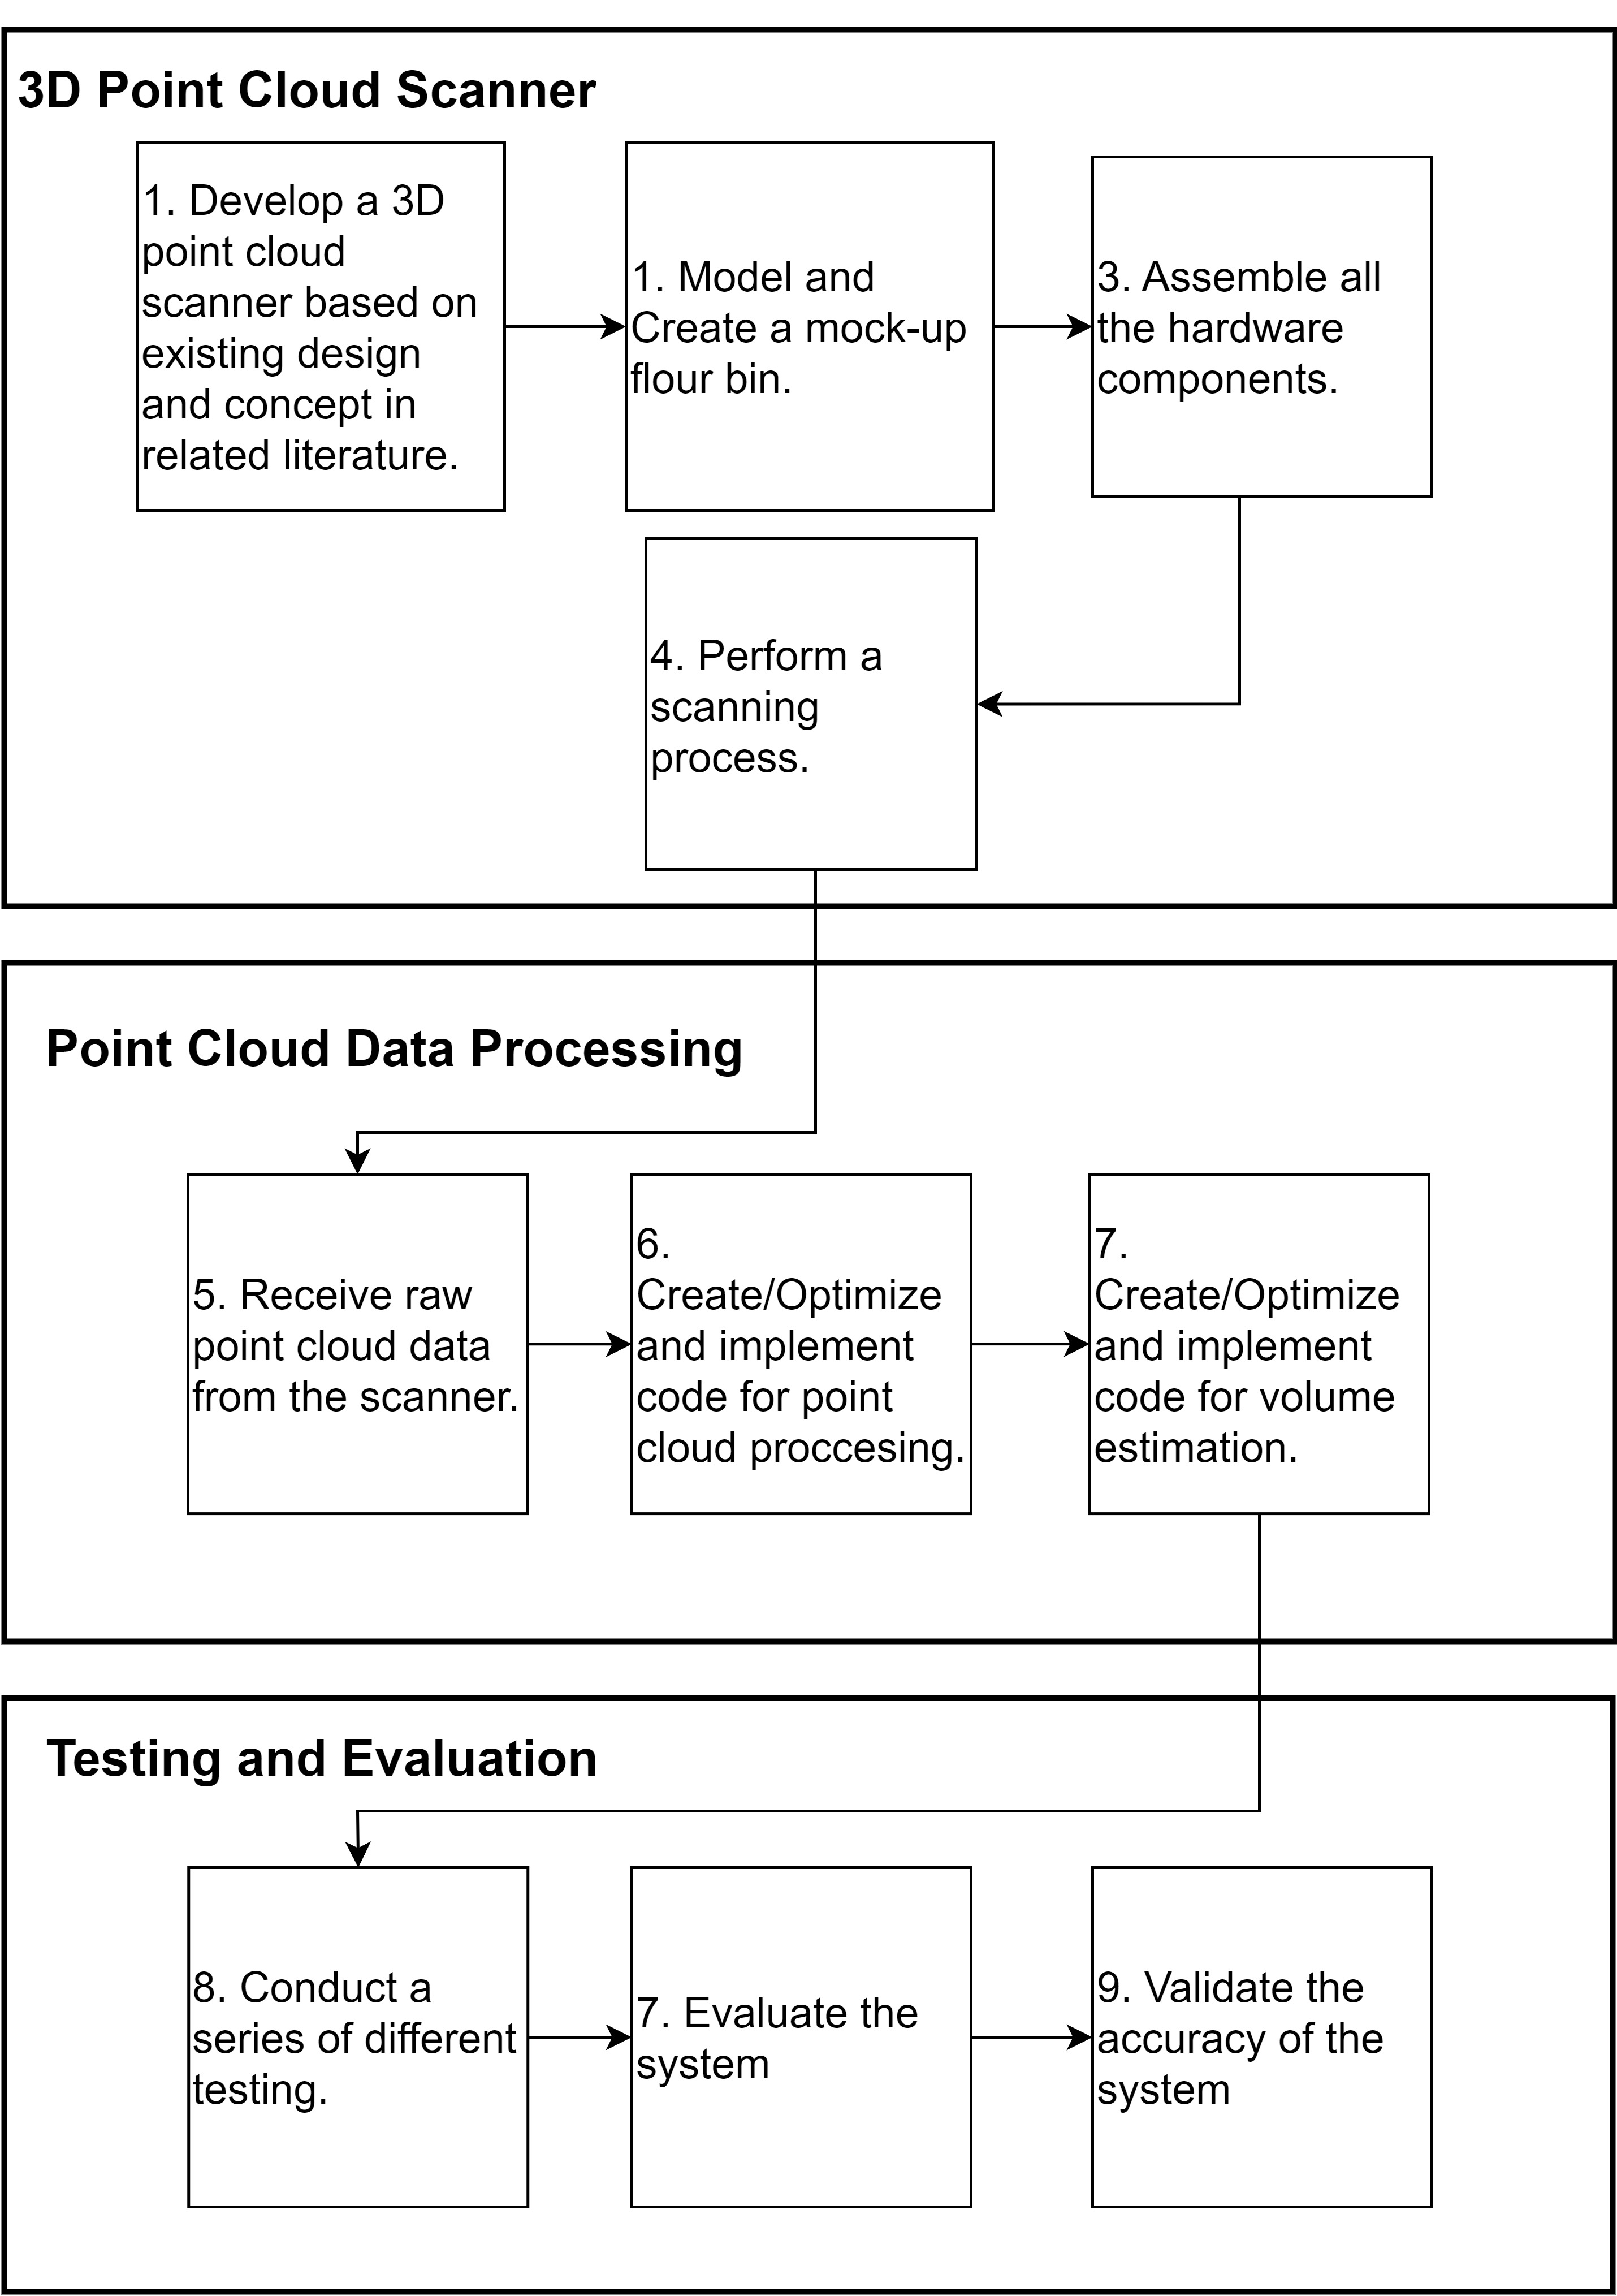
\includegraphics[width=0.9\textwidth, height=0.7\textheight]{conceptual-framework-2}
	\caption{General Conceptual Flow}
	\label{fig:conceptual-framework}
\end{figure}

\section{Theoretical Framework}
\label{intro:sec:Theoretical Framework}
The research is based on the idea of using automation for industrial operations, specifically in the food industry. Point cloud data is a collection of an unorganized set of x, y, and z coordinates in a three-dimensional space. There are various ways to acquire point cloud data, and one possible way is through active non-contact sensing technology such as LiDAR sensor. LiDAR uses Time-of-Flight (TOF) method of measuring distance between the sensor to the object. TOF scanners are inexpensive compared to other specialized 3D scanners \citep{chua2017}. The researcher will utilize LiDAR to acquire 3D point cloud data because of its ability to gather points data and converts them into a global world coordinate frame \citep{bi2021}. The study does, however, acknowledge the potential limits of LiDAR, when the environment is prone to medium (e.g., water vapor, gases, dust particle, etc.) that can obstruct the target surface, the LiDAR acquired point cloud data that may alter the precision of the data \citep{chua2017}. Thus, the researcher will manage the raw point cloud data by filtering the factoring medium such as dust. Lastly, Delaunay Triangulation is a computational geometry computation that connects a set points to form a mesh of triangles. It can be used for volume estimation by calculating the volume of a convex hull which will be use in this study.

\section{Definition of Terms}
\label{intro:sec:Definition of Terms}

\begin{enumerate}
	\item \textbf{LiDAR} \textemdash stands for Light Detection and Ranging, can also be describe as Light Imaging, Detection, and Ranging. It is a method for determining ranges by targeting an object or a surface with a laser and measuring the time-of-flight to determine the distance.

	\item \textbf{Bin} \textemdash is a large container used to store materials, such as grain, coal, sand, or other bulk goods. They are typically made of metal, plastic, or wood and come in various sizes, shapes, and designs.

	\item \textbf{ROS} \textemdash Robot Operating System is a set of open-source libraries and tools designed to help developers build robot applications. It provides a common framework for creating, managing and sharing code, data, and other resources related to robotic systems.

	\item \textbf{Point Cloud} \textemdash is a set of data points in a three-dimensional space, typically representing the surface of an object. Each point in the cloud is defined by its three-dimensional coordinates (x, y, and z) and may also include additional information such as color, intensity, or normal vector.
	\item \textbf{Convex Hull} \textemdash is the minimum convex polygon from the set of points that encompasses all of the points in the set.

\end{enumerate}